\documentclass{article}

\usepackage{titlesec}
\newcommand{\sectionbreak}{\clearpage}

\usepackage{fancyhdr}
\pagestyle{fancy}
\lhead{Emanuel Casiano-Diaz}
\rhead{CSYS300: PoCS - Homework 02 - 09/15/2018}
\renewcommand{\headrulewidth}{0.4pt}
\renewcommand{\footrulewidth}{0.4pt}

\usepackage{amsmath}
\usepackage{amssymb}
\usepackage{bm}
\usepackage{pdfpages}

\usepackage{enumerate}% http://ctan.org/pkg/enumerate

\usepackage{hyperref}
\hypersetup{
    colorlinks=true,
    linkcolor=blue,
    filecolor=magenta,      
    urlcolor=cyan,
}


\begin{document}

\section{Exercise 1}

Code used throughout the assignment can be found in the following git repository: \url{https://github.com/ecasiano/PrinciplesOfComplexSystems} \\
\\
Normalization Constant:

\[
\begin{aligned}
\int_{-\infty}^{+\infty} P(x) dx &= c \int_{a}^{b} x^{-\gamma} \\
&= c \frac{x^{-\gamma + 1} \vert_{x=a}^{x=b} }{ (-\gamma + 1)} \\
&= \frac{c}{(-\gamma + 1)} (b^{-\gamma+1} - a^{-\gamma+1}) = 1 \text{ ; normalization condition} \\ 
\implies c &= \frac{-\gamma+1}{(b^{-\gamma+1} - a^{-\gamma+1})}
\end{aligned}
\]

where $0 < a \leq x \leq b$ and $\gamma > 1$. \\
\\
Condition on gamma: \\

The reason that the condition $\gamma > 1$ is imposed is to make the integral $\int_{a}^{b} x^{-\gamma} dx$ convergent. It may help to recall a well-known series, the p-series: $\sum_{n=1}^{\infty} \frac{1}{n^p}$. This series converges only when $p>1$. Note that this is none other than a discrete version of the integral we're dealing with. Then, by extension, the integral should only converge for $\gamma > 1$ too, which is nice since we would like to keep probabilities finite.
 
 \section{Exercise 2}

For a continuous and random variable $X$, the $n^{th}-$moment of the distribution is defined as:

\[ \mu_{n} = \int_{-\infty}^{+\infty} x^n P(x) dx\]

where $n = 1,2,3,...$. Then substituting the given probability distribution:
\[
\begin{aligned}
\mu_{n} &= (\frac{-\gamma+1}{b^{-\gamma+1} - a^{-\gamma+1}}) \int_{a}^{b} x^{-\gamma+n} dx \\
&= (\frac{-\gamma+1}{b^{-\gamma+1} - a^{-\gamma+1}}) \frac{x^{-\gamma+n+1}\vert_{x=a}^{x=b}}{-\gamma+n+1} \\
&= (\frac{-\gamma+1}{b^{-\gamma+1} - a^{-\gamma+1}}) \frac{b^{-\gamma+n+1} - a^{-\gamma+n+1}}{-\gamma+n+1} \\
\mu_n &= (\frac{-\gamma+1}{-\gamma+n+1}) (  \frac{b^{-\gamma+n+1} - a^{-\gamma+n+1}}{b^{-\gamma+1} - a^{-\gamma+1}}    )
\end{aligned}
\]

\section{Exercise 3}

Want: $\lim_{b\to\infty} \mu_n$ as a function of gamma. 
\\
Depending on the size of $\gamma$, the sign of the exponent ($-\gamma+n+1$) in the expression for $\mu_n$ will change. Three cases for gamma will be evaluated: \\
\\
Case 1: $\gamma > (n+1)$ \\
\\
In this case , since $(-\gamma+n+1) < 0$ , then $\lim_{b\to \infty} b^{-\gamma+n+1} = 0$. \\
\\
Case 2: $\gamma < (n+1)$ \\
\\
In this case , since $(-\gamma+n+1) > 0$ , then $\lim_{b\to \infty} b^{-\gamma+n+1} = \infty $. \\
\\
Case 3: $\gamma = (n+1)$ \\
\\
In this case , since $(-\gamma+n+1) = 0$ , then $\lim_{b\to \infty} b^{-\gamma+n+1} = 1$. \\
\\
Additionally in the limit of $b\to\infty$, we have that $a^{-\gamma+n+1} \to a^{-\gamma+n+1}$, $a^{-\gamma+1} \to a^{-\gamma+1}$ and $b^{-\gamma+1} \to 0$ (since $\gamma > 1$ and the exponent is thus negative). Substituting these limiting values for each term, the $n^{th}-$moment as $b\to\infty$ can be described by the function:

\[ \lim_{b\to\infty} \mu_n = \begin{cases}
(\frac{-\gamma+1}{-\gamma+n+1}) a^n & \gamma > (n+1) \\
\infty & \gamma < (n+1) \\
0 & \gamma = (n+1) \\
\end{cases}\] \\
\\
Note that for the above limit to be finite, $\gamma \geq n+1$.

\section{Exercise 4}

Assume that $b \gg a$. Depending on the conditions on $\gamma$ discussed in the previous exercise: $\gamma > (n+1)$, $\gamma < (n+1)$ and $\gamma = (n+1)$, the dominating term in the expression will vary. Again, each case will be evaluated: \\
\\
Case 1: $\gamma > (n+1)$ and $b \gg a$ \\
\\
In this case , since $(-\gamma+n+1) < 0$, then $b^{-\gamma+n + 1} -a^{-\gamma+n+1} \approx -a^{-\gamma+n+1}$\\
\\
Case 2: $\gamma < (n+1)$ and $b \gg a$ \\
\\
In this case , since $(-\gamma+n+1) > 0$, then $b^{-\gamma+n + 1} -a^{-\gamma+n+1} \approx b^{-\gamma+n+1}$\\
\\
Case 3: $\gamma = (n+1)$ and $b \gg a$\\
\\
In this case , since $(-\gamma+n+1) = 0$, then $b^{-\gamma+n + 1} -a^{-\gamma+n+1} = 1 - 1 = 0$\\
\\
Additionally, when $b\gg a$, we have that $b^{-\gamma + 1} - a^{-\gamma+1} \approx - a^{-\gamma+1}$ (since $-\gamma + 1 < 0$). Substituting these estimates, the $n^{th}-$moment as a function of $\gamma$ is approximately:

\[ \mu_n \approx \begin{cases}
(\frac{-\gamma+1}{-\gamma+n+1}) a^n & \gamma > (n+1) \\
(\frac{-\gamma+1}{-\gamma+n+1}) \frac{-b^{-\gamma+n+1}}{a^{-\gamma+1}} \text{(number with a very large magnitude)} & \gamma < (n+1) \\
0 & \gamma = (n+1)\\
\end{cases}\]

\section{Exercise 5}

NOTE: In this section, the standard deviation, $\sigma$, of the continuous random variable $X$ should be found. Nevertheless, most of the following lines will be expressed in terms of the variance, $\sigma^2$, to avoid having a large radical all over the expressions cluttering things up.\\
\\
The variance can be expressed in terms of the first and second moments as:
\[ \sigma^2 = \mu_2 - \mu_1^{2}\]
\\
Recall the generating function for the $n^{th}-$moment:
\[ \mu_n = (\frac{-\gamma+1}{-\gamma+n+1}) (  \frac{b^{-\gamma+n+1} - a^{-\gamma+n+1}}{b^{-\gamma+1} - a^{-\gamma+1}}    ) \]
\\
Thus, substituting $n=2$ and $n=1$ for the second and first moments, respectively, in the $\sigma^2$ equation, it is seen that:
\[ \sigma^2 = (\frac{-\gamma+1}{-\gamma+3}) (  \frac{b^{-\gamma+3} - a^{-\gamma+3}}{b^{-\gamma+1} - a^{-\gamma+1}}    ) - (\frac{-\gamma+1}{-\gamma+2})^2 (  \frac{b^{-\gamma+2} - a^{-\gamma+2}}{b^{-\gamma+1} - a^{-\gamma+1}}    )^2\]
\\
To check this result, the form of the variance as $b$ tends to infinity has been hinted as being:

\[ \lim_{b\to\infty} \sigma^2 = \frac{(\gamma-c_1)}{(\gamma-c_2)(\gamma-c_3)} a^2\]
\\
where the constants $c_1,c_2$ and $c_3$ have to be determined. Imposing the convergence condition $\gamma \geq n+1 = 2  + 1 = 3$, the limit of the variance as $b$ tends to infinity becomes:

\[ \lim_{b\to\infty} \sigma^2 = \frac{(\gamma-1)}{(\gamma-3)(\gamma-2)} a^2 \]
\\
which has the same form as the hint. \\
\\
Near the end of the allowed range on $\gamma$, that is $\gamma \to 3$, note that the above limit will blow up. In other words:

\[ \lim_{\gamma\to 3} \left [ \lim_{b\to \infty} \sigma ^2 \right ] = \infty \]
\\
Thus, for infinitely large $b$, the variance and the standard deviation blow up as $\gamma$ gets close to the end of it's allowed range!

\section{Exercises 6}

\begin{figure}[h!]
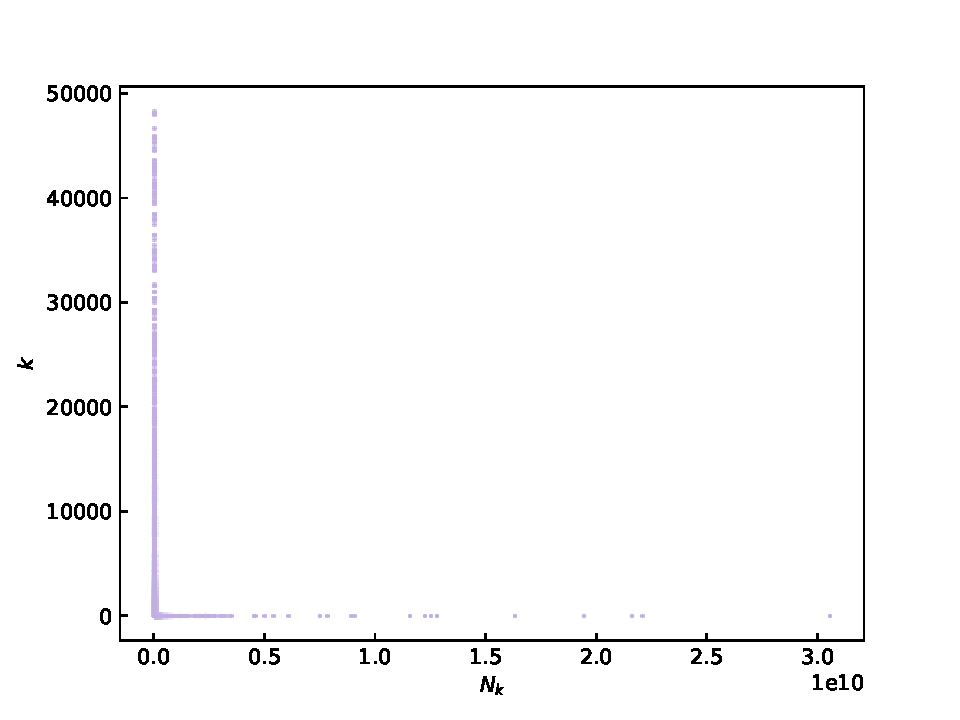
\includegraphics[width=\linewidth]{Q06/wordFrequency.pdf}
\caption{Frequency $k$ that groups of $N_k$ words are repeated in a Google data set}
\label{fig:words}
\end{figure}

\begin{figure}[h!]
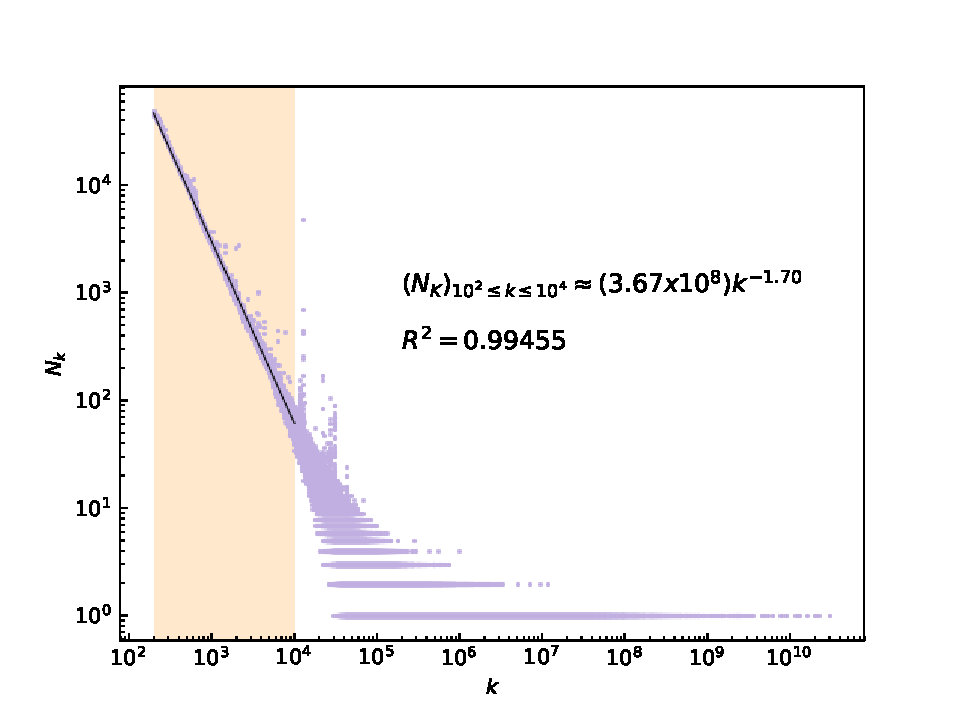
\includegraphics[width=\linewidth]{Q06/wordFrequencyLog.pdf}
\caption{Frequency $k$ that groups of $N_k$ words are repeated in a Google data set plotted in a base 10, log-log scale. The orange region denotes where power-law scaling holds (via "eye-balling"). By doing a linear regression on the sets $\log_{10} N_k$  ($y-$values) and $\log_{10} k$ ($x-$values) only inside the orange region, the prefactor and scaling exponent have been estimated to be $A \approx 3.67 x 10^{8}$ and $p \approx -1.70$, respectively.}
\label{fig:envelope}
\end{figure}

NOTE: ***Exercise 7 has been answered in the figure caption***


\section{Exercise 7}

***Answered in caption of the previous figure***

\section{Exercise 8}

The following values are statistical measures corresponding to the set of values $N_k$ for all $k$, not only the orange region: \\
\\
Mean: 56.7418\\
Variance: 827320.5566\\
Standard Deviation: 909.5716\\
\\
Do these make sense according to the theory developed in the homework? \\
\\
First off, this data set follows a distribution of the same form as the one proposed in Exercise 1, so the theory developed in Exercises 2-5 should hold for the distribution $N_k$.  \\
\\
Second, consider the lower and upper bounds of $k$: $k_{low} = 2.00x10^2$ and $k_{high} = 3.06x10^{10}$. These bounds are 8 orders of magnitude apart, thus we can assume that $k_{high} \gg k_{low}$. The power law exponent has a value of $p =  1.70 < 3$. Thus, basing off the estimates from Exercise 4, the $n^{th}-$moment of this distribution should be a large number that grows exponentially with increasing moment order. Recall that $\sigma^2 = \mu_2 - \mu_1^2$, thus it makes sense that the variance obtained is so large, due to the large size of $\mu_2$. \\
\\
There is one discrepancy only, and that is unfortunately the mean. By estimating the first moment based off the Exercise 4 prediction, I expected $\mu_1 \approx 1.3x10^6$. This is evidently not the case. Further investigation will be required to learn the cause but one thing to look at is at how good this power law exponent is to describe the whole set. This is a heavy-tailed distribution and perhaps the tail needs to be cleaned up.
\\

\section{Exercise 9}

Two girls? \\
\\
Possible combinations assuming one of the children is a girl: Girl-Boy, Boy-Girl, Girl-Girl. There is only one combination in which there's two girls out the three possible combination. Thus, the probability of having another girl after having already one is: 1/3. \\
\\
Two girls? First one born on a Tuesday? \\
\\
Probability of having another girl = 13/27
 


\end{document}